% L12c lecture companion. Notebook hashes and coverage are recorded in README.md.
% Style files and Cornell seal are copied unchanged from the L12a deck (identical
% to L10c, L10a, L9c, and L9a, which match the approved L6a deck). The Q-table
% figure is the L12a lecture's SVG, converted to a light PDF by `make figures`;
% the Q-networks figure is the light TikZ PDF in ../figs/Fig-Q-Networks.
%
% Notation follows the lecture: the Q-network Q(s,a;theta) with parameters theta,
% the target network theta^-, the action set A with n actions, the feature vector
% phi(s) in R^p, the weight vectors w_a and weight matrix W, basis-function centers c_j and
% width sigma, transitions (s_i,a_i,r_i,s_i',d_i) with done flag d_i, targets y_i,
% the loss L(theta), the learning rate alpha, the discount factor gamma, the
% replay buffer D of size M, the warm-up size N_warm, the mini-batch size N_batch,
% the copy interval C, the exploration probability epsilon, the random number rho,
% the number of episodes N, the step limit t_max, and the counters t and tau.
\documentclass[aspectratio=169,11pt]{beamer}
\usepackage{vnslides}
\renewcommand{\vnlecturecode}{L12c}
\newcommand{\lecturelink}{https://github.com/varnerlab/CHEME-5800-CourseRepository-Fall-2026/blob/main/weeks/week-12/L12c/CHEME-5800-L12c-Lecture-DeepQLearning-Fall-2026.ipynb}
\newcommand{\examplelink}{https://github.com/varnerlab/CHEME-5800-CourseRepository-Fall-2026/blob/main/weeks/week-12/L12c/CHEME-5800-L12c-Example-LinearDQN-AdaptiveDosing-Fall-2026.ipynb}
\newcommand{\lablink}{https://github.com/varnerlab/CHEME-5800-CourseRepository-Fall-2026/blob/main/weeks/week-12/L12d/CHEME-5800-L12d-Lab-DoubleDQN-Fall-2026.ipynb}
\newcommand{\lecturesource}[1]{\note{[Sources]\par
  \href{\lecturelink}{L12c lecture: Deep Q-Learning.}\par
  #1\par[/Sources]}}
\newcommand{\Aset}{\mathcal A}
\newcommand{\Dset}{\mathcal D}
\newcommand{\Nbatch}{N_{\text{batch}}}
\newcommand{\Nwarm}{N_{\text{warm}}}

\title{\texorpdfstring{{\vnheavy L12c}: Deep Q-Learning}{L12c: Deep Q-Learning}}
\subtitle{\texorpdfstring{Q-networks and the DQN algorithm\\[3pt]CHEME 5800 Cornell University}{Q-networks and the DQN algorithm; CHEME 5800 Cornell University}}
\author{Copyright Jeffrey Varner 2026. All Rights Reserved}

\begin{document}
\special{pdf:minorversion 7}
\vntitlepage

\begin{frame}{Objectives for Today}
  How can an agent learn action values when its states are too many for a table?

  \vspace{0.4em}
  {\large\textbf{\ink{Today's concepts}}}
  \vspace{0.2em}
  \begin{itemize}\setlength{\itemsep}{0.4em}
    \item \hilite{Explain the limits of a Q-table}: the number of states
      grows exponentially with the number of state variables, and a table
      learns nothing about a state from the states around it.
    \item \hilite{Write the DQN loss and its gradient step}: deep Q-learning
      fits a Q-network to targets built from its own estimates, and tabular
      Q-learning is a special case.
    \item \hilite{Describe the replay buffer and the target network}: each one
      addresses a problem of Q-learning with a network.
  \end{itemize}
  \slidenote{Lecture:}{\href{\lecturelink}{Deep Q-Learning}}
  \lecturesource{Introduction and three Learning Objectives.}
\end{frame}

\begin{frame}{Lecture and Example}
  \textbf{\ink{Lecture:}}
  \href{\lecturelink}{Deep Q-Learning}

  In this lecture, we replace the Q-table with a function that computes the
  action values from a few numbers that describe the state. This idea is the
  basis of deep Q-learning and of its best-known method, the deep Q-network
  (DQN). We start with the simplest such function, a linear one.

  \vspace{1.1em}
  \textbf{\ink{Example:}}
  \href{\examplelink}{Learn a dosing policy without a grid using a linear DQN}

  In this example, an agent learns to dose the patient of the dosing lab
  without rounding the tumor burden and the toxicity to grid levels. Its linear
  Q-network has 148 weights, where the dosing lab's Q-table has 6,724 entries.
  \lecturesource{Introduction and the Examples section.}
\end{frame}

\begin{frame}{The Q-Table}
  Tabular Q-learning stores one action value for every state-action pair.

  \vspace{0.2em}
  \centering
  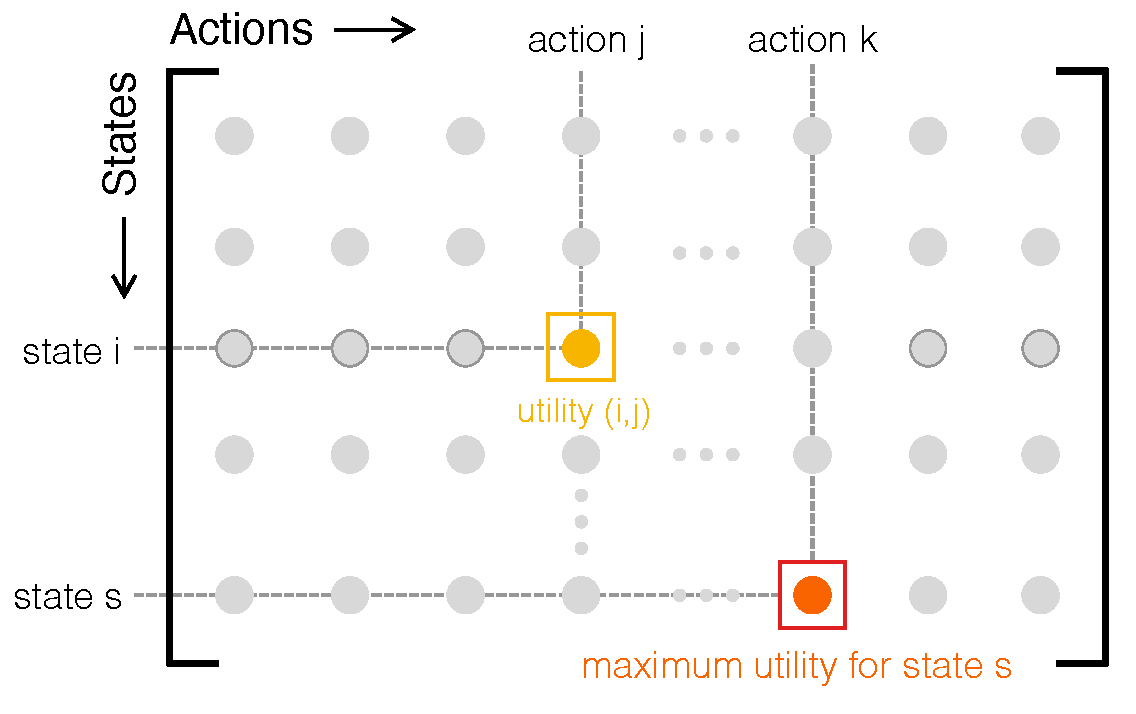
\includegraphics[width=\textwidth,height=0.50\paperheight,keepaspectratio]{assets/Fig-Q-Schematic.pdf}

  \vspace{0.2em}
  \raggedright
  Entry $(i,j)$ holds the value (utility) of taking action $j$ in state $i$.
  The policy reads each row and picks the column with the largest entry.
  \lecturesource{The Curse of Dimensionality: the Q-table caption and figure.
    Figure: ../../L12a/figs/Fig-Q-Schematic.svg, converted to a light PDF.}
\end{frame}

\begin{frame}{The Curse of Dimensionality}
  The Q-table has three problems:

  \vspace{0.3em}
  \begin{itemize}\setlength{\itemsep}{0.5em}
    \item \hilite{The table grows exponentially}: a state with $m$ variables,
      each rounded to $L$ levels, has $L^{m}$ states. The dosing-lab patient
      has $41^{2}=1681$ states, but ten variables would give about
      $1.3\times10^{16}$.
    \item \hilite{The table does not generalize}: each entry learns only from
      visits to its own state-action pair. Two states with almost the same
      tumor burden share nothing.
    \item \hilite{Rounding changes the problem}: the dosing lab's policy gives
      no dose at a tumor burden of 0.109, because its grid rounds 0.109 to
      0.100, a level that counts as a cure.
  \end{itemize}

  \vspace{0.5em}
  Richard Bellman called this exponential growth the
  \href{https://en.wikipedia.org/wiki/Curse_of_dimensionality}{curse of dimensionality}.
  \lecturesource{The Curse of Dimensionality: the three problems and the closing sentence.}
\end{frame}

\begin{frame}{Q-Networks}
  Instead, we replace the table with a function that computes the action values
  from a few numbers that describe the state.

  \vspace{0.4em}
  A \hilite{Q-network} is a function $Q(s,a;\theta)$ with adjustable parameters
  $\theta$. It takes a state $s$ as its input and returns one Q-value for each
  of the $n$ actions in the action set $\Aset=\{a_{1},\dots,a_{n}\}$. The
  greedy policy picks the action with the largest entry:
  \[
    \pi(s)=\arg\max_{a\in\Aset}Q(s,a;\theta)
  \]

  Learning now means adjusting $\theta$ instead of the entries of a table. The
  number of parameters is set by the network, not by the number of states.
  \lecturesource{The Curse of Dimensionality: closing sentence. Q-Networks: definition, greedy policy, and the closing paragraph.}
\end{frame}

\begin{frame}{Two Q-Networks}
  \centering
  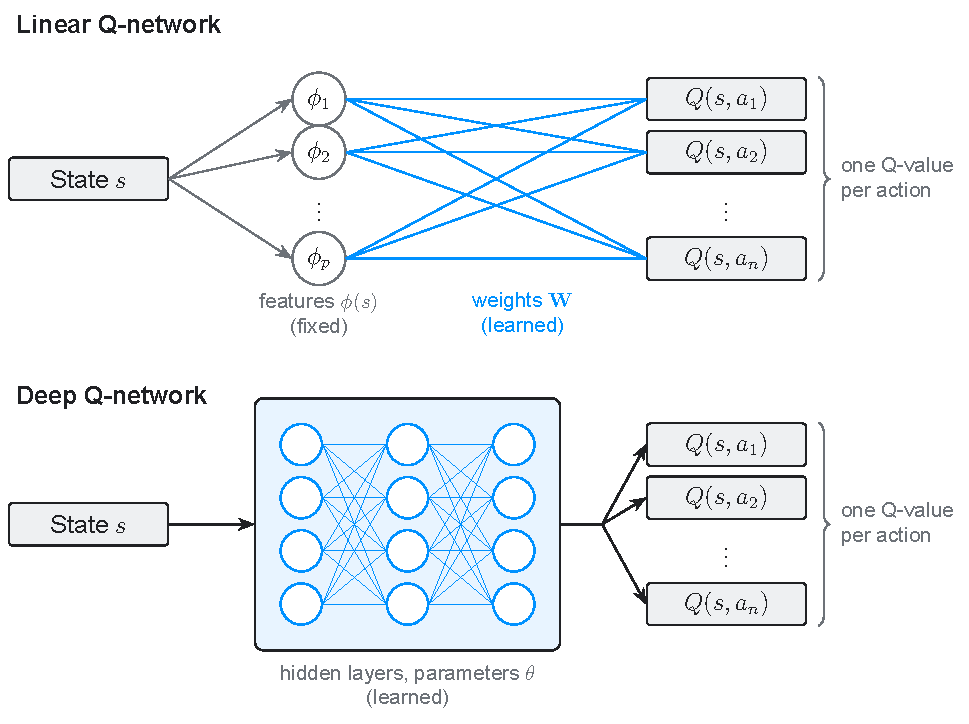
\includegraphics[width=\textwidth,height=0.60\paperheight,keepaspectratio]{assets/Fig-Q-Networks.pdf}

  \vspace{0.2em}
  \raggedright
  In the linear network, the $p$ features $\phi_{1}(s),\dots,\phi_{p}(s)$ are fixed,
  and only the weights (blue) are learned. In the deep network, the hidden
  layers are learned as well.
  \lecturesource{Q-Networks: the Two Q-networks figure and caption.
    Figure: ../figs/Fig-Q-Networks/Fig-Q-Networks.pdf (light TikZ build).}
\end{frame}

\begin{frame}{A Linear Q-Network}
  A linear Q-network describes the state $s$ by a \hilite{feature vector}
  $\phi(s)\in\mathbb R^{p}$, a list of $p$ numbers computed from the state.
  The Q-value of action $a$, a weighted sum of the features with weight vector
  $\mathbf w_{a}\in\mathbb R^{p}$, is given by:
  \[
    Q(s,a;\mathbf W)=\mathbf w_{a}^{\top}\phi(s)=\sum_{j=1}^{p}w_{a,j}\,\phi_{j}(s)
  \]

  where $w_{a,j}$ is the weight of action $a$ on feature $\phi_{j}(s)$. The
  weight matrix $\mathbf W$ has one row $\mathbf w_{a}^{\top}$ per action,
  which gives $n\cdot p$ weights in all.
  \lecturesource{A linear Q-network: definition, equation, and the weight matrix.}
\end{frame}

\begin{frame}{Two Choices of Features}
  In the example, the state is $s=(B,Z)$, the tumor burden and the toxicity.

  \vspace{0.8em}
  \begin{columns}[T,onlytextwidth]
    \begin{column}{0.48\textwidth}
      \textbf{\ink{Radial basis functions}} with centers
      $\mathbf c_{j}$ and width $\sigma$:
      \[
        \phi_{j}(s)=\exp\left(-\frac{\lVert s-\mathbf c_{j}\rVert_{2}^{2}}{2\sigma^{2}}\right)
      \]
      where $\lVert s-\mathbf c_{j}\rVert_{2}$ is the distance from $s$ to
      $\mathbf c_{j}$. Nearby states get similar Q-values. What the agent
      learns in one state carries over to its neighbors.
    \end{column}
    \begin{column}{0.48\textwidth}
      \textbf{\ink{One-hot}}: number the states, and put a one in entry $s$
      and zeros everywhere else:
      \[
        Q(s,a;\mathbf W)=w_{a,s}\vphantom{\frac{\lVert s\rVert_{2}^{2}}{2\sigma^{2}}}
      \]
      The weight matrix $\mathbf W$ is the transpose of the Q-table. A Q-table
      is a linear network.
    \end{column}
  \end{columns}
  \lecturesource{A linear Q-network: The features paragraph and basis-function equation, the nearby-states sentence, and A Q-table is a linear network.}
\end{frame}

\begin{frame}{A Deep Q-Network}
  A \hilite{neural network} is a function built from layers. A
  \hilite{deep Q-network} replaces the fixed features with the
  \hilite{hidden layers} of a neural network, the layers between its input and
  its output:

  \vspace{0.3em}
  \begin{itemize}\setlength{\itemsep}{0.5em}
    \item Each hidden layer is a column of \hilite{units}. Each unit takes a
      weighted sum $x$ of its inputs and passes it through a fixed nonlinear
      function, such as $\max(0,x)$. The hidden layers learn their own
      features from the data.
    \item The output layer takes weighted sums only, which lets a Q-value be
      negative.
    \item \href{https://www.nature.com/articles/nature14236}{Mnih et al. (2015)}
      trained a deep Q-network to play Atari video games from the pixels on the
      screen.
  \end{itemize}

  \vspace{0.5em}
  The rest of this lecture holds for any Q-network with parameters $\theta$,
  the weights $\mathbf W$ in the linear case.
  \lecturesource{A deep Q-network: all three paragraphs.}
\end{frame}

\begin{frame}{The DQN Loss}
  Q-learning moves the entry $Q(s,a)$ toward the target
  $r+\gamma\max_{a'}Q(s',a')$, where $r$ is the reward, $s'$ is the next
  state, and $\gamma$ is the discount factor. A
  Q-network has no entry to move:

  \vspace{0.3em}
  \begin{itemize}\setlength{\itemsep}{0.5em}
    \item Deep Q-learning adjusts $\theta$ to shrink the squared gap between the
      network's prediction and the target. This fit is a \hilite{regression}
      with the targets as labels.
    \item The targets are called \hilite{bootstrap targets}, because they are
      built from the network's own estimates.
    \item The training data are \hilite{transitions}
      $(s_{i},a_{i},r_{i},s_{i}',d_{i})$: a state, the action taken, the reward,
      the next state, and a \hilite{done flag} $d_{i}$. The flag is one if
      $s_{i}'$ is \hilite{absorbing}, a state that ends the episode for good,
      and zero otherwise.
  \end{itemize}

  \vspace{0.5em}
  In the example, a cure and a toxic death are absorbing. An episode that stops
  at a step limit keeps $d_{i}=0$ on its last transition.
  \lecturesource{The DQN Loss: the four paragraphs before the box.}
\end{frame}

\begin{frame}{DQN Bellman Loss}
  The target $y_{i}$ of transition $i$ is the value that the prediction
  $Q(s_{i},a_{i};\theta)$ should match:
  \[
    y_{i}=r_{i}+\gamma\,(1-d_{i})\max_{a'\in\Aset}Q(s_{i}',a';\theta^{-})
  \]
  where $\theta^{-}$ are the parameters of the \hilite{target network}, a
  delayed copy of the Q-network. The factor $(1-d_{i})$ drops the future value
  when $s_{i}'$ is absorbing.

  \vspace{0.4em}
  On a \hilite{mini-batch} of $\Nbatch$ past transitions, the loss is half the
  mean of the squared \hilite{prediction errors} $y_{i}-Q(s_{i},a_{i};\theta)$:
  \[
    \mathcal L(\theta)=\frac{1}{2\Nbatch}\sum_{i=1}^{\Nbatch}\left(y_{i}-Q(s_{i},a_{i};\theta)\right)^{2}
  \]
  The prediction uses the action $a_{i}$ that was actually taken. The target
  uses the best next action under the target network.
  \lecturesource{The DQN Loss: the DQN Bellman Loss box.}
\end{frame}

\begin{frame}{The Gradient Step of a Linear Network}
  One step of \hilite{gradient descent} with learning rate $\alpha$ is
  $\theta\gets\theta-\alpha\nabla_{\theta}\mathcal L(\theta)$, where the
  gradient $\nabla_{\theta}\mathcal L$ is the vector of derivatives of the loss
  and $\alpha$ sets the size of the step.

  \vspace{0.4em}
  For the linear network, the derivative of the prediction
  $\mathbf w_{a_{i}}^{\top}\phi(s_{i})$ with respect to $\mathbf w_{a_{i}}$ is
  the feature vector $\phi(s_{i})$. The target $y_{i}$ comes from the target
  network and does not depend on $\mathbf W$. One step updates the row of each
  action in the mini-batch:
  \[
    \mathbf w_{a}\gets\mathbf w_{a}+\frac{\alpha}{\Nbatch}\sum_{i\,:\,a_{i}=a}\left(y_{i}-\mathbf w_{a}^{\top}\phi(s_{i})\right)\phi(s_{i})
  \]

  \vspace{0.4em}
  \textbf{\ink{A check against the table}}: with one-hot features, a mini-batch
  that holds only the transition just taken, and $\theta^{-}=\theta$ at every
  step, this update is the tabular Q-learning update.
  \lecturesource{The DQN Loss: the gradient descent paragraph. The gradient step of a linear network: the derivative, the update of row a, and A check against the table. The comparison with logistic regression and the Q-learning update equation are left out.}
\end{frame}

\begin{frame}{Two Stabilizers}
  Tabular Q-learning converges when every non-absorbing state-action pair is
  visited infinitely often, and the learning rates of each pair add up to
  infinity while their squares add up to a finite number. Deep
  Q-learning can instead \hilite{diverge}, with values that grow without bound
  (\href{http://incompleteideas.net/book/the-book-2nd.html}{Sutton and Barto,
  2018}). It adds two stabilizers:

  \vspace{0.3em}
  \begin{itemize}\setlength{\itemsep}{0.5em}
    \item \hilite{The replay buffer}: many gradient steps on consecutive
      transitions fit one region of states and spoil the values elsewhere. The buffer $\Dset$ keeps
      the last $M$ transitions, and each training step uses a random
      mini-batch of $\Nbatch$ of them.
    \item \hilite{The target network}: if the Q-network computed its own
      targets, each gradient step would also move them. A copy of the
      Q-network, $Q(s,a;\theta^{-})$, computes the targets instead, and every
      $C$ steps the algorithm copies $\theta^{-}\gets\theta$.
  \end{itemize}

  \vspace{0.5em}
  Between copies, training is close to a regression on random examples with
  fixed labels.
  \lecturesource{DQN Algorithm and Stabilizers: the opening paragraph, the two stabilizer bullets, and the closing paragraph.}
\end{frame}

\begin{frame}{DQN Algorithm: Initialize}
  \textbf{Initialize}: Given a Q-network $Q(s,a;\theta)$, set $\theta$ to zeros
  for a linear network or to small random values for a deep network, and copy
  the parameters to the target network, $\theta^{-}\gets\theta$. Start with an
  empty replay buffer $\Dset$ and a total step counter $\tau\gets0$.

  \vspace{0.5em}
  \textbf{Hyperparameters}:
  \begin{itemize}\setlength{\itemsep}{0.2em}
    \item the discount factor $0\le\gamma<1$ and the learning rate $\alpha>0$,
    \item the exploration probability $\epsilon$ of each episode,
    \item the number of episodes $N$ and the maximum number of steps per episode $t_{\max}$,
    \item the buffer size $M$ and the \hilite{warm-up} size $\Nwarm$, the
      number of transitions the buffer must hold before training begins,
    \item the mini-batch size $\Nbatch$ and the target-network copy interval $C$.
  \end{itemize}
  \lecturesource{Algorithm: Initialize and Hyperparameters.}
\end{frame}

\begin{frame}{DQN Algorithm}
  \small
  For each of the $N$ episodes \textbf{do}:
  \begin{enumerate}\setlength{\itemsep}{0.1em}
    \item Choose a starting state $s$ that is not absorbing, and set the step
      counter $t\gets0$.
    \item While $s$ is not absorbing and $t<t_{\max}$ \textbf{do}:
      \begin{enumerate}\setlength{\itemsep}{0.1em}
        \item Choose the action $a$: draw a random number $\rho$ uniformly from $[0,1]$.
          \begin{itemize}\setlength{\itemsep}{0em}
            \item If $\rho\le\epsilon$ \textbf{then} choose $a\in\Aset$
              uniformly at random (exploration).
            \item Otherwise, choose the greedy action
              $a\gets\arg\max_{a'\in\Aset}Q(s,a';\theta)$ (exploitation).
          \end{itemize}
        \item Take action $a$, and observe the reward $r$, the next state $s'$,
          and the done flag $d$ from the \emph{world}, where $d=1$ if $s'$ is
          absorbing and $d=0$ otherwise.
        \item Store the transition $(s,a,r,s',d)$ in the replay buffer $\Dset$,
          and remove the oldest transition if $\Dset$ holds more than $M$.
        \item Update the counters, $t\gets t+1$ and $\tau\gets\tau+1$.
        \item If $\Dset$ holds at least $\Nwarm$ transitions \textbf{then} take
          one training step.
        \item If $\tau$ is a multiple of $C$ \textbf{then} copy the Q-network
          to the target network, $\theta^{-}\gets\theta$.
        \item Update the state, $s\gets s'$.
      \end{enumerate}
  \end{enumerate}

  \vspace{0.1em}
  \textbf{Extract Policy}: For any state $s$, compute
  $\pi(s)\gets\arg\max_{a\in\Aset}Q(s,a;\theta)$.
  \lecturesource{Algorithm: the For/While pseudocode and Extract Policy. The sub-steps of the training step are on the next slide.}
\end{frame}

\begin{frame}{DQN Algorithm: The Training Step}
  \small
  Step 2.5 of the loop takes one training step:
  \begin{enumerate}\setlength{\itemsep}{0.4em}
    \item Draw a mini-batch of $\Nbatch$ transitions
      $(s_{i},a_{i},r_{i},s_{i}',d_{i})$, $i=1,\dots,\Nbatch$, uniformly at
      random with replacement from $\Dset$.
    \item Compute the target of each transition with the \emph{target network},
      $y_{i}\gets r_{i}+\gamma\,(1-d_{i})\max_{a'\in\Aset}Q(s_{i}',a';\theta^{-})$.
    \item Compute the loss on the actions that were actually taken:
      \[
        \mathcal L(\theta)=\frac{1}{2\Nbatch}\sum_{i=1}^{\Nbatch}\left(y_{i}-Q(s_{i},a_{i};\theta)\right)^{2}
      \]
    \item Take a \emph{single} gradient descent step on the loss,
      $\theta\gets\theta-\alpha\nabla_{\theta}\mathcal L(\theta)$.
      \begin{itemize}
        \item \emph{Why only a single step?} Many steps on one small mini-batch
          can overfit its few transitions and undo what the network learned
          from the rest of the buffer.
      \end{itemize}
  \end{enumerate}
  \lecturesource{Algorithm: the four sub-steps of step 5 of the While loop, with the note under the gradient step.}
\end{frame}

\begin{frame}{Notes on the Algorithm}
  \begin{itemize}\setlength{\itemsep}{0.7em}
    \item The policy gives an action for any state, including states the agent
      never visited.
    \item \emph{Why random starting weights for a deep network?} If all the
      weights start equal, the units of a hidden layer compute the same feature,
      get the same update, and stay equal. A linear network has fixed
      features, and zeros work.
    \item In the example, a linear network with 36 basis functions and a constant feature trains
      for 3,000 episodes in about one second. The same algorithm trains a deep
      network, which needs a package for neural networks and much more time.
  \end{itemize}
  \lecturesource{Algorithm: the sentence after Extract Policy, the note on random starting weights, and the paragraph on training time.}
\end{frame}

\begin{frame}{Example: A Linear DQN for Adaptive Dosing}
  In this example, an agent learns to dose the patient of the dosing lab
  without a grid:

  \vspace{0.5em}
  \begin{enumerate}\setlength{\itemsep}{0.5em}
    \item Build the patient model, with the tumor burden and the toxicity kept
      as continuous numbers.
    \item Train a linear DQN with 36 basis functions and a constant feature, 148 weights
      in all.
    \item Compare its doses with value iteration on the dosing lab's 41-level
      grid and on a 201-level grid.
  \end{enumerate}

  \vspace{0.5em}
  From the dosing lab's starting state, the linear DQN cures the patient in 23 cycles
  and the 201-level policy in 19. The 41-level policy does not cure the patient within 100 cycles.
  \slidenote{Example:}{\href{\examplelink}{A linear DQN for adaptive drug dosing}}
  \lecturesource{Algorithm: the example box. Companion example: Tasks 1--3 and the key takeaways.}
\end{frame}

\begin{frame}{Overestimation}
  The DQN target uses the largest estimated Q-value of the next state:

  \vspace{0.3em}
  \begin{itemize}\setlength{\itemsep}{0.5em}
    \item Every estimate has some error, and the largest one is often an
      estimate whose error is positive.
    \item The target then tends to be too high on average, even when each estimate is
      right on average. This upward bias is called \hilite{overestimation}.
    \item Overestimation spreads back to the values of earlier states, and it
      can make a worse action look like the best one.
  \end{itemize}
  \lecturesource{Overestimation: the first two paragraphs.}
\end{frame}

\begin{frame}{Double DQN}
  The maximum uses the same estimates to choose the next action and to score
  it. \hilite{Double DQN}
  (\href{https://arxiv.org/abs/1509.06461}{van Hasselt, Guez, and Silver, 2016})
  chooses with the Q-network and scores with the target network. Its target is
  given by:
  \[
    y_{i}=r_{i}+\gamma\,(1-d_{i})\,Q\Bigl(s_{i}',\;\arg\max_{a'\in\Aset}Q(s_{i}',a';\theta);\;\theta^{-}\Bigr)
  \]

  The target network is a recent copy of the Q-network, and the two share part
  of their errors. Double DQN can reduce overestimation, but it does not always
  remove it.
  \lecturesource{Overestimation: the Double DQN paragraph, its target, and the closing paragraph.}
\end{frame}

\begin{frame}{Lab: Overestimation and Double DQN}
  In the \href{\lablink}{lab}, we'll measure overestimation and watch it make
  Q-learning and DQN prefer the worse action on a small problem with two
  states:

  \vspace{0.5em}
  \begin{itemize}\setlength{\itemsep}{0.5em}
    \item Measure how far the largest of several noisy estimates lands above
      the true largest value.
    \item Compare Q-learning with Double Q-learning, which keeps two Q-tables
      that score each other's choices.
    \item Test Double DQN, and measure how often it still prefers the worse
      action and how that depends on how often we copy the target network.
  \end{itemize}
  \slidenote{Lab:}{\href{\lablink}{Overestimation and Double DQN}}
  \lecturesource{Lab section. Lab notebook: introduction, Learning Objectives, and Tasks 1--3.}
\end{frame}

\begin{frame}{Summary}
  We replaced the Q-table with a Q-network and built deep Q-learning around it.

  \vspace{0.5em}
  {\large\textbf{\ink{Key takeaways}}}
  \vspace{0.3em}
  \begin{itemize}\setlength{\itemsep}{0.6em}
    \item \textbf{\ink{Q-networks.}} A Q-network computes every action value
      from features of the state, with a fixed number of parameters.
    \item \textbf{\ink{The DQN loss.}} Deep Q-learning fits the network by
      regression on bootstrap targets from the target network.
    \item \textbf{\ink{Stabilizers.}} Random mini-batches from the replay
      buffer and a fixed target network make training steadier.
  \end{itemize}

  \vspace{0.5em}
  A linear network with well-chosen features is often enough for a problem with
  a few state variables. A deep network learns its own features, which lets the
  same algorithm work from raw inputs such as images.
  \lecturesource{Summary: three key takeaways and the closing paragraph.}
\end{frame}

\end{document}
